\documentclass{article}
\usepackage{graphicx}
\usepackage[utf8]{inputenc} % allow utf-8 input
\usepackage[T1]{fontenc}    % use 8-bit T1 fonts
\usepackage{hyperref}       % hyperlinks
\usepackage{url}            % simple URL typesetting
\usepackage{booktabs}       % professional-quality tables
\usepackage{amsfonts}       % blackboard math symbols
\usepackage{nicefrac}       % compact symbols for 1/2, etc.
\usepackage{amsmath}
\usepackage{microtype}      % microtypography
\usepackage{geometry}
\usepackage{subfigure}
%\usepackage{showframe}%

\newgeometry{vmargin={20mm}, hmargin={15mm,15mm}}   % set the margins
\renewcommand{\figurename}{Slika}
   \newtheorem{theorem}{Teorem}
\numberwithin{equation}{section}

\renewcommand*\contentsname{Sadržaj}

\title{Skripta za Fiziku Čvrstog Stanja I}


\author{Adrian Udovičić, Vinko Sršan}

\begin{document}
\maketitle
\pagenumbering{roman}
\section*{\centering Uvod}

Svrha ove skripte je upoznati studente smjera Fizike Čvrstog Stanja sa sadržajem istoimenog kolegija. Nadam se da će vam pomoći. Ukoliko želite dodati nešto slobodno se javite da vas ubacim u projekt.

\vfill

\begin{center}
\tableofcontents
\end{center}
\vfill
\newpage
%% početak prvog poglavlja
\pagenumbering{arabic}
\section{Kristalne Strukture}
\subsection{Općenite definicije}
Neke definicije u FČS.
\paragraph{Translacija vektora rešetke}
Idealna rešetka napravljena je od identičnih grupa atoma. Grupa se zove \textbf{baza}. \textbf{Rešetka} je skup točaka vezanih za bazu. 3D rešetku opisujemo s primitivnim vektorima $\mathbf{a_1}$ , $\mathbf{a_2}$ , $\mathbf{a_3}$  tako da raspored atoma u rešetci izgleda isto iz točke \textbf{r} kao i iz točke  
\begin{equation}
    \mathbf{r'} =  \mathbf{r} + u_1 \mathbf{a_1} + u_2 \mathbf{a_2} + u_3 \mathbf{a_3}.
    \label{EQ1}
\end{equation}
Gdje su $u_i \in \mathbb{Z}$ ; i= 1, 2, 3. Skup $\mathbf{r'}$ definira točke rešetke. 
Rešekta je \textbf{primitivna} ako bilo koje dvije točke rešetke ($\mathbf{r'}$ i $\mathbf{r}$), koje zadovoljavaju jednadžBudu 
\ref{EQ1} izgledaju isto. Najmanji volument čelije je definiran s $\mathbf{a_1} \cdot \mathbf{a_2} \times \mathbf{a_3}$. 
Translacija rešetke definirana je pomakom kristala za vekotor translacije kristala. \footnote{Top Kek} 
\begin{equation}
    \mathbf{T}=u_1\mathbf{a_1}+u_2\mathbf{a_2}+u_1\mathbf{a_3}.
    \label{EQ2}
\end{equation}
Bilo  koje dvije točke rešetke su spojene s vektorom ovog oblika. 

\paragraph{Baza i kristalna struktura}

Bazu kristala možemo identificirati kad odredimo primitivne vektore. 
\begin{figure}[h!]
    \centering
    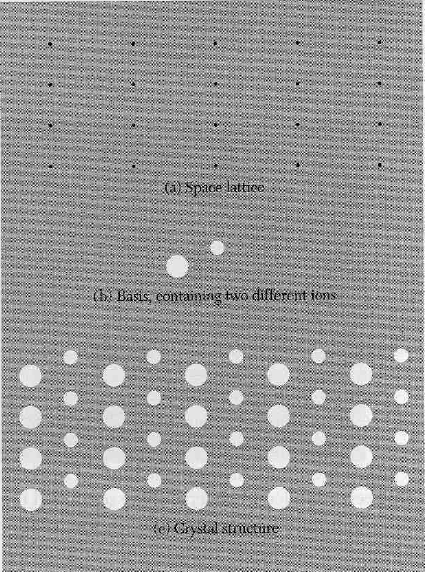
\includegraphics[width=7cm]{Slika_1.PNG}
    \caption{Kristalna rešetka + Baza = Kristalna struktura}
    \label{fig:S1}
\end{figure}Slika \ref{fig:S1} pokazuje kako se dobiva kristal tako da dodajemo bazu svakoj točki. Svaka baza nekog kristala je identična jedna drugoj s obzirom na kompoziciju, orijentaciju i raspored. 
Položaj atoma \textit{j} je određen sljedećom jednadžbom.
\begin{equation}
    \mathbf{r}_{j}=x_{j} \mathbf{a}_{1}+y_{j} \mathbf{a}_{2}+z_{j} \mathbf{a}_{3}
    \label{EQ3}
\end{equation}
\paragraph{Primitivna čelija rešetke}
Paralelopiped definiran s primitivnim vektorima (koji \underline{nisu jedinstveni}!) $\mathbf{a_1}$, $\mathbf{a_2}$, $\mathbf{a_3}$ 
zove se \textbf{primitivna čelija}. Kao i primitivni vektori, čelija također onda nije jedinstvena! Volumen je već poznat i iznosi 
$\mathbf{V_c}=\left|\mathbf{a_1} \cdot \mathbf{a_2} \times \mathbf{a_3}\right|$. 
Nijedna baza ne sadrži manje atoma nego što sadrži čelija primitivne baze. Još jedan način određivanja primitivne čelije je pomoću 
\textbf{Wigner-Seitz čelije} (Slika \ref{fig:S2}).
\begin{figure}[h!]
    \centering
    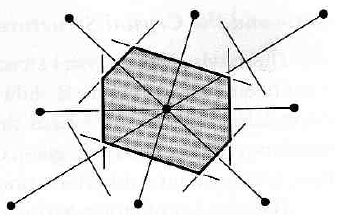
\includegraphics[width=7cm]{Slika_2.PNG}
    \caption{Wigner-Seitz čelija}
    \label{fig:S2}
\end{figure}

\newpage
\subsection{Osnovni tipovi rešetaka}
Pomoću vektora translacije \textbf{T} kristalne rešetke se mogu prenositi ili mapirati. Tipična operacija simetrije je rotacija po osi koja prolazi kroz čvor rešetke.  Postoje jedno-, dvo-, tro-, četvero- i šeterorotirajuće transformacije vraćaju rešetku u prvobitni položaj ($2\pi$, $\frac{2\pi}{2}$, $\frac{2\pi}{3}$, $\frac{2\pi}{4}$, $\frac{2\pi}{6}$). Za sad nije pronađena rešetka s peterorotirajućim translacijama ove prirode. Kao primjer evo slika \ref{fig:S3}.
\begin{figure}[h!]
    \centering
    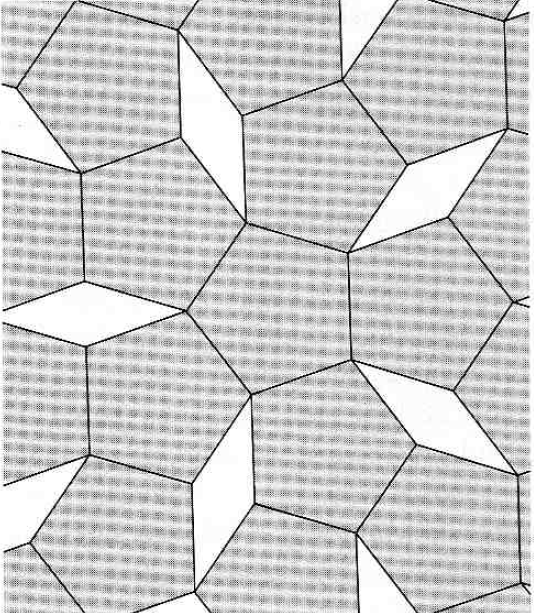
\includegraphics[width=9cm]{Slika_3.PNG}
    \caption{Peterostruka os simetrije kristalne rešetke. Ima praznog (bijelo) prostora.}
    \label{fig:S3}
\end{figure}
Grupa točaka rešetke je skup simetričnih operacija koje kada se vrše na nekoj točki rešetke vraćaju rešetku u prvobitno stanje, tj. rešetka izgleda kao da se ništa nije promijenilo. 
\paragraph{Tipovi 2D rešetke}
Postoji beskonačan broj mogućih rešetki pošto nema ograničenja na duljinu transformacijskih vektora rešetke, ili kuta $\phi$ između njih. Rešetka na \ref{fig:S4} je napravljena pomoću proizvoljnih izbora primitivnih vektora. 
\newpage
\begin{figure}[h!]
    \centering
    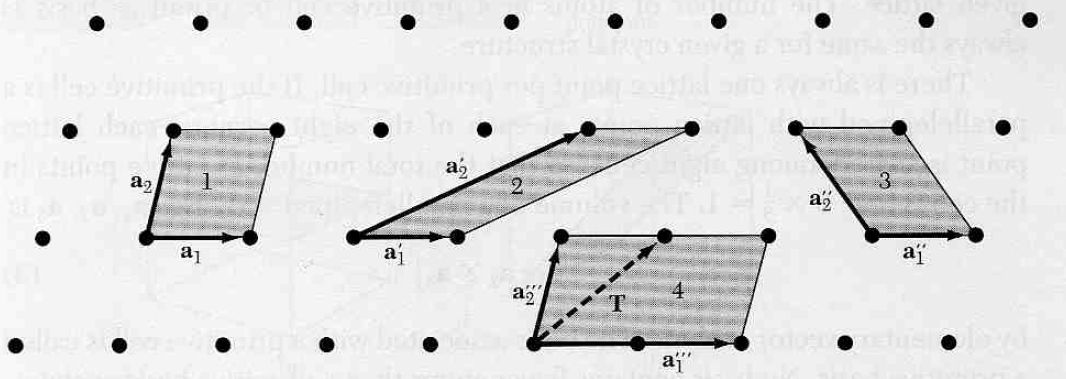
\includegraphics[width=15cm]{Slika_3a.PNG}
    \caption{Sve kombinacije su validne osim '4' jer $\mathbf{a}'''_1$ i $\mathbf{a}'''_2$ nisu primitivni vektori.}
    \label{fig:S4}
\end{figure}
To su ujedno i najopčenitije 2D rešetke. Zove se nagnuta rešetka i invarijantna je na $\pi$ i $2\pi$ rotacije oko bilo koje točke rešetke. Postoje 5 vrsta 2D rešetki prikazane na slici \ref{fig:S5}. \textbf{Bravais rešetka} je fraza za određenu vrstu rešetku. 

\begin{figure}[h!]
    \centering
    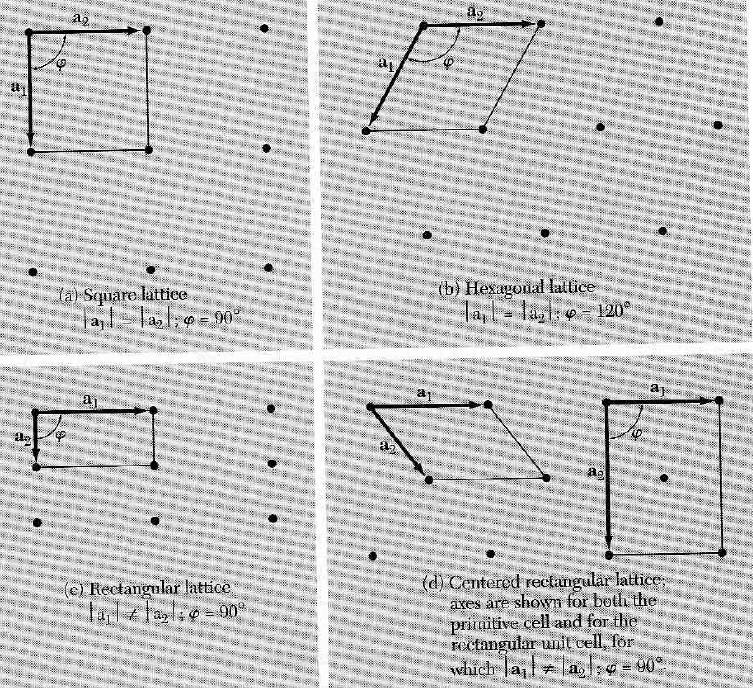
\includegraphics[width=10cm]{Slika_4.PNG}
    \caption{5 vrsta 2D rešetki.}
    \label{fig:S5}
\end{figure}
\newpage
\paragraph{Tipovi 3D rešetke}
U 3 dimenzije potrebno je 14 različitih tipova rešetki. Osnovna je triklinička. Klasificiraju se po 7 tipova čelija navedenih na slici \ref{fig:S6}. 

\begin{figure}[h!]
    \centering
    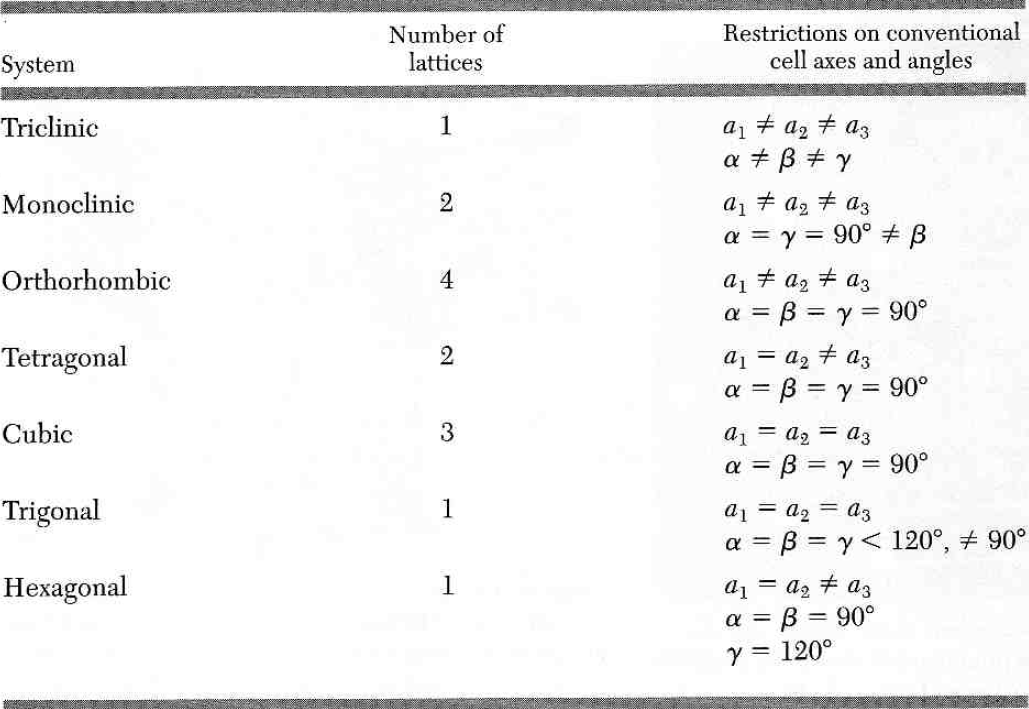
\includegraphics[width=10cm]{Slika_5.PNG}
    \caption{14 vrsti 3D rešetki.}
    \label{fig:S6}
\end{figure}
Čelije na slici \ref{fig:S7} su kubne od kojih je samo SC primitivna, a na slici \ref{fig:S8} se nalaze karakteristike svake od njih.
%% dvije slike
\begin{figure}[h!]
    \centering
    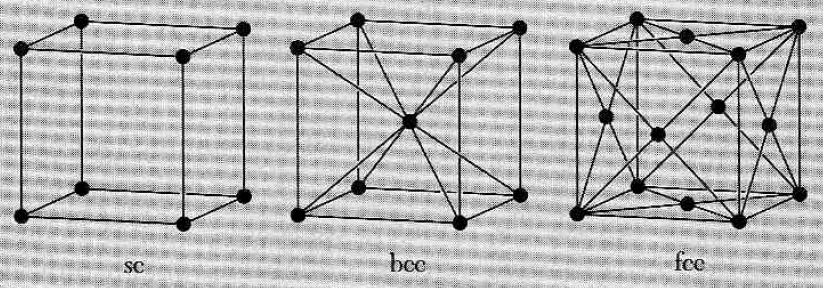
\includegraphics[width=10cm]{Slika_6.PNG}
    \caption{Tipovi kubične rešetke.}
    \label{fig:S7}
\end{figure}

\begin{figure}[h!]
    \centering
    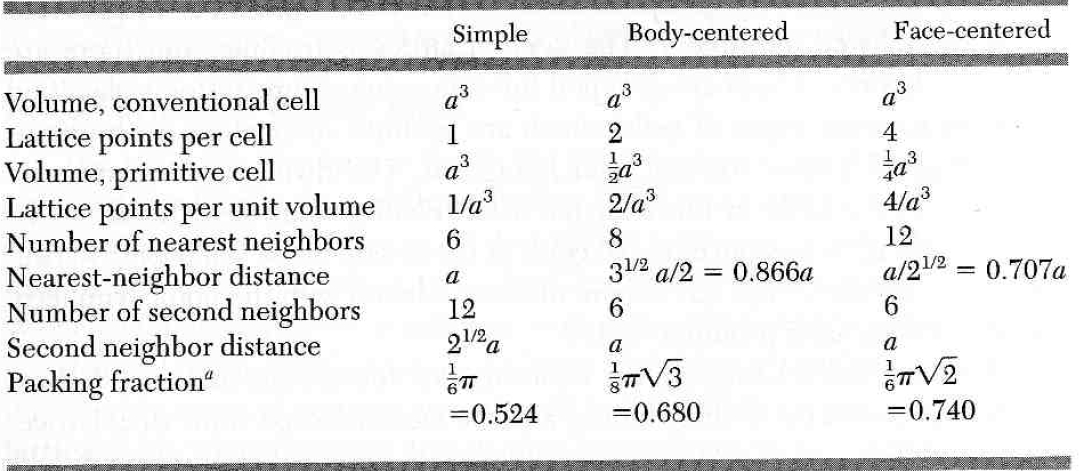
\includegraphics[width=10cm]{Slika_7.PNG}
    \caption{Karakteristike rešetki sa slike \ref{fig:S7}.}
    \label{fig:S8}
\end{figure}
\paragraph{Bravais rešetka}
Osnovni koncept kristalnih rešetaka je \underline{Bravais rešetka}.Ona opisuje gemetriju periodične strukture.  Dvije ekvivalentne definicje su: 
\begin{itemize}
    \item Bravais rešetka je beskonačni niz diskretnih točaka koje izgledaju identično iz koje god pozicije iz gledamo.
    \item 3D Bravais rešetka opisana je vektorom položaja \textbf{R} oblika 
    \begin{equation}
        \mathbf{R}= n_1\mathbf{a}_1 + n_2\mathbf{a}_2 + n_3\mathbf{a}_3,
        \label{EQ3b}
    \end{equation}
\end{itemize}
gdje su $a_i$; i=1, 2, 3, primitivni vektori. Naravno, očito je da su jednadžbe \ref{EQ2}, \ref{EQ3} i \ref{EQ3b} identične.
\paragraph{Indeksi kristalnih ravnina}
Orijentaciju ravnine određuju 3 točke na ravnini, s uvjetom da nisu kolinearne. Bolje je koristiti indekse određene presjecanjem ravnine s \underline{primitivnim} osima. Način dobivanja \textbf{Millerovih indeksa} je sljedeći: Nađu se točke ravnine koje presijecaju primitivne osi $a_i$; i=1, 2, 3, te se uzme recipročna vrijednost tih brojeva. Zadnji korak je reduciranje tih razlomaka na cijele brojeve.  Primjer je dan na slici \ref{fig:S9} tako da ravnina presijeca osi $a_i$ u točkama 3, 2 i 2. Zapišemo ih kao razlomak $\frac{1}{3}$,  $\frac{1}{2}$, i $\frac{1}{2}$. Nađemo najmanjeg zajedničkog djelitelja brojeva u nazivniku, što je u ovom slučaju 6, i pomnožimo s njim da dobijemo Millerove indekse, u ovom slučaju 2, 3 i 3, te ih zapišemo kao $\left( 2, 3, 3\right)$.
\begin{figure}[h!]
    \centering
    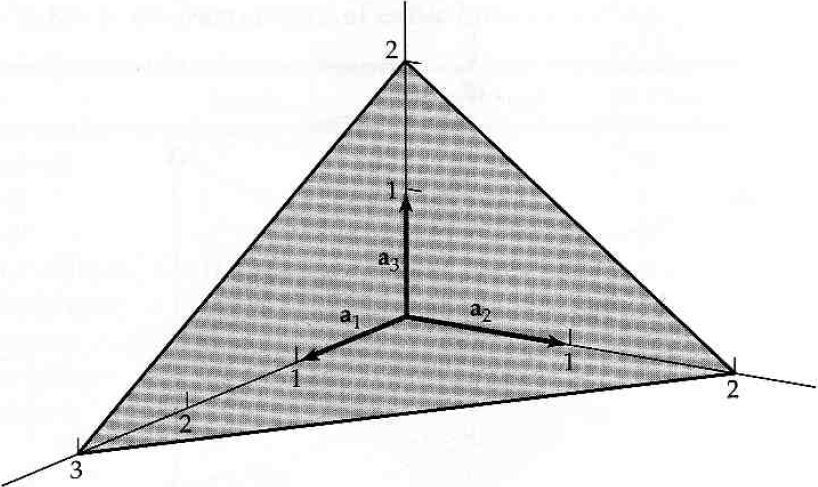
\includegraphics[width=10cm]{Slika_8.PNG}
    \caption{Primjer dobivanja Millerovih indeksa.}
    \label{fig:S9}
\end{figure}

\newpage
\section{Ogib valova i recipročna rešetka}
\paragraph{Braggov zakon}

\begin{figure}[h!]
    \centering
    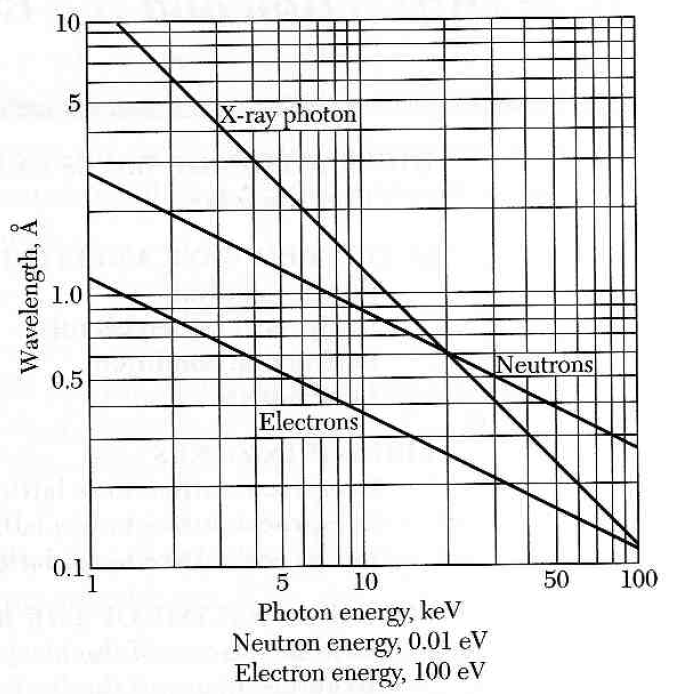
\includegraphics[width=10cm]{Slika_9.PNG}
    \caption{Energije i valne duljine za fotone, elektrone i neutrone}
    \label{fig:S10}
\end{figure}
Braggov zakon možemo opisati pomoću kristalne rešetke na način da kristalne ravnine na međusobnoj udaljenosti \textit{d}, ozračujemo svjetlošću valne duljine $\lambda$ pod nekim kutem $\alpha$. Razlika puteva dviju zraka je onda $2dsin(\alpha)$. Da bi interakcija bila konstruktivna, razlika puteva za zraku mora biti proporcionalna cjelobrojnom višekratniku valne duljine, tj. mora vrijediti Braggov zakon (slika \ref{bragg}).
\begin{figure}[h!]
    \centering
    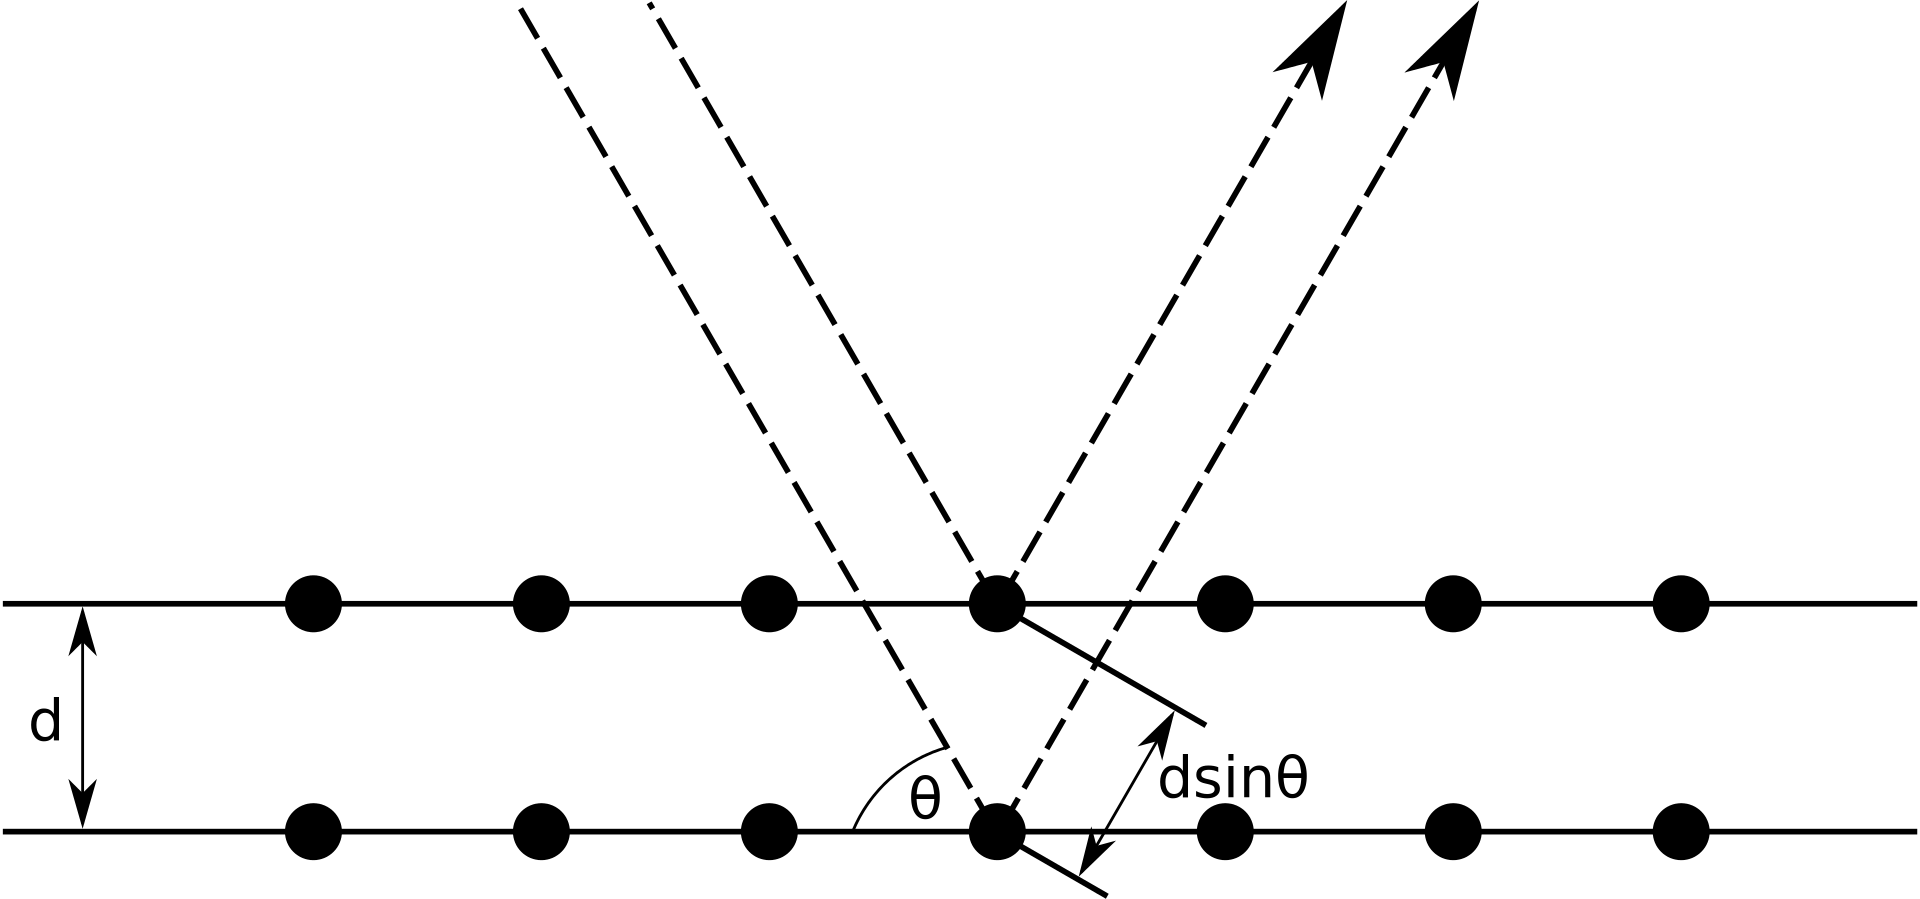
\includegraphics[width=10cm]{Bragg1.png}
    \caption{Bragg difrakcija, zamislite da piše $d sin(\alpha)$}
    \label{bragg}
\end{figure}
Braggov zakon je posljedica periodične strukture rešetke. Iako Braggov zakon ne ovisi o sastavu baze, kompozicija baze određuje intenzitet različitih redova difrakcije. 
\subsection{Amplituda raspršenja}
Za određivanje amplitude raspršenja prvo moramo imati prostornu raspodjelu elektrona u čeliji. Prije smo saznali da je bilo koje lokalno svojstvo kristala (koncentracija naboja, gustoća elektrona, gustoća magnetskog momenta,..) invarijantno na transformacije rešetke oblika \textbf{T} napisano kao u \ref{EQ2}. Gustoća elektrona n(\textbf{r}) je periodična funkcija od \textbf{r} s periodom \textbf{$a_1$}, \textbf{$a_2$}, \textbf{$a_3$}, pa n(\textbf{r}+\textbf{T})=n(\textbf{r}). U jednoj dimenziji Fourierov transformat od n(x) glasi 
\begin{equation}
    n(x)= n_0 + \sum_{p>0}\left[ C_p cos\left(\frac{2\pi p}{a}x\right)+ S_p sin\left(\frac{2\pi p}{a}x\right)\right],
    \label{EQ2_1}
\end{equation}
gdje je p$\in$ $\mathbb{N}$,a $ C_p$ i $S_p$ $\in$ $\mathbb{R}$. Slijedi: 
\begin{equation}
    n(x)= n_0 + \sum_{p>0}\left[ C_p cos\left(\frac{2\pi p}{a}x + 2\pi p \right)+ S_p sin\left(\frac{2\pi p}{a}x + 2\pi p\right)\right],
    \label{EQ2_2}
\end{equation}
Koristeći formule za kosinus i sinus zbroja \footnote{$sin(x \pm y)= sin(x) cos(y) \pm cos(x) sin(y)$ \\ $cos(x\pm y)= cos(x) cos(y) \mp sin(x) sin(y)$} dobivamo opet jednadžbu \ref{EQ2_1}.\\ Točke $\frac{2\pi p}{a}$ nam kažu koji su dozvoljeni članovi u Fourierovom redu tj. član je dozvoljen ako je konzistentan s periodičnošću kristala.  Fourierov transformat možemo i kompaktnije napisati: 
\begin{equation}
n(x)=\sum_{p=-\infty}^{+\infty}n_p e^{i \frac{2\pi p}{a}x},
    \label{EQ2_3}
\end{equation}
gdje je $n_p$ $\in \mathbb{C}$. Da osiguramo da nam n(x) ostane realan određujemo $n_{-p}^*=n_p$, tj. 
\begin{equation}
n_p\left(cos(\phi) + isin(\phi)\right)+ n_{-p}\left( cos(\phi) - isin(\phi)\right) = \left(n_p + n_{-p}\right)cos(\phi)+ i\left(n_p-n_{-p} \right) sin(\phi)
    \label{EQ2_4}
\end{equation} 
što je jednako realnoj funkciji 
\begin{equation}
2Re\left\{ n_p \right\} cos(\phi) - 2Im\left\{ n_p\right\}sin(\phi)
    \label{EQ2_5}
\end{equation}
   Za trodimenzionalni Fourierov transformat od $n(\textbf{r})$ je oblik 
   \begin{equation}
       n(\textbf{r})=\sum_G n_G e^{i \textbf{G}\textbf{r}}
       \label{EQ2_6}
   \end{equation}
   gdje samo treba pronaći vektore \textbf{G} koji su invarijantni na transformaciju.
   Skup Fourierovih koeficijenata $n_G$ određuje amplitudu raspršenja rendgenskih zraka. \\
   Inverzija Fourierovog reda daje da su $n_p$ dobiveni iz 
   \begin{equation}
       n_p=a^{-1}\int_0 ^a dx n(x)e^{-i\frac{2\pi p}{a}x}
       \label{EQ2_7}
   \end{equation}
   \paragraph{Dokaz} Uvrštavanjem n(x) u $n_p$ iz \ref{EQ2_3} dobivamo 
   \begin{equation}
       n_p=a^{-1}\sum_{p'}n_{p'}\int_o ^a dx e^{\frac{2\pi p}{a}x \cdot(p'-p)}
   \end{equation}
   Za $p'\neq p $integral iznosi $\frac{a}{i 2 \pi (p'-p)}(e^{i 2 \pi (p'-p)}-1)=0$, pošto su 
	 p' i p cijeli brojevi, a $e^{i 2\pi (cijeli broj)}=1$. Za $p' = p$ integral je jednak $a$, jer je $e^{i 0}=1$,
	 t.d. $n_p=a^{-1}n_p a= n_p$, što je identitet, tako da je \ref{EQ2_7} identitet. Isto vrijedi za $n\left(\mathbf{r}\right)$.\hfill $\square$
   \subsection{Vektori recipročne rešetke}
   Recipročna rešetka je Fourierov transformat Bravaisove rešetke. Ako su $\mathbf{a_1}$, $\mathbf{a_2}$ i $\mathbf{a_3}$ primitivni vektori onda su primitivni vektori recipročne rešetke dani kao: 
 
     \begin{equation}
     \begin{split}
\mathbf{b_1}&=2\pi \frac{\mathbf{a_2}\times \mathbf{a_3}}{V},  \\
\mathbf{b_2}&=2\pi \frac{\mathbf{a_3}\times \mathbf{a_1}}{V}, \\
\mathbf{b_3}&=2\pi \frac{\mathbf{a_1} \times\mathbf{a_2}}{V}, \\
     \end{split}
   \end{equation}
   gdje je $V=\mathbf{a_1}\cdot \mathbf{a_2}\times \mathbf{a_3}$ volumen primitivne čelije. Vrijedi $\mathbf{a_i}\cdot\mathbf{b_j}=2 \pi \delta_{ij}$.
   Točke recipročne rešetke su dane skupom vektora 
   \begin{equation}
       \mathbf{G}=\sum_{i=1}^3v_i\mathbf{b_i}
   \end{equation}.
   $\mathbf{G}$ nazivamo vektorom recipročne rešetke. Vektori $\mathbf{G}$ u \ref{EQ2_6} su isti ti vektori.
   \paragraph{Dokaz}
   Neka je $\mathbf{T}=\sum_{i=1}^3 u_i \mathbf{a_i}$ pa je $n(\mathbf{r+T})=\sum_G n_G e^{i\mathbf{G}\cdot \mathbf{r}}e^{i\mathbf{G}\cdot \mathbf{T}}$. 
   Odavdje dobivamo $\mathbf{G\cdot T}=\left(\sum_{i=1}^3v_i b_i\right)\cdot \left(\sum_{i=1}^3 u_i a_i \right) = 2\pi \left(\sum_i^3 u_i v_i \right)$, 
	 tj. dobivamo $e^{i\mathbf{G \cdot T}}=1$, jer su $u_i$ i $v_i$ cijeli brojevi.\\
	 Slijedi da je $n(\mathbf{r+T})=\sum_G n_G e^{i\mathbf{G \cdot T}}=n(\mathbf{r})$. \hfill $\square$
   
   \subsection{Difrakcijski uvjeti}
\begin{theorem}
   Skup vektora recipročne rešetke $\left\{ \mathbf{G}\right\}$ određuje moguće difrakcijske uzorke. 
\end{theorem}
   \begin{figure}[h!]
       \centering
       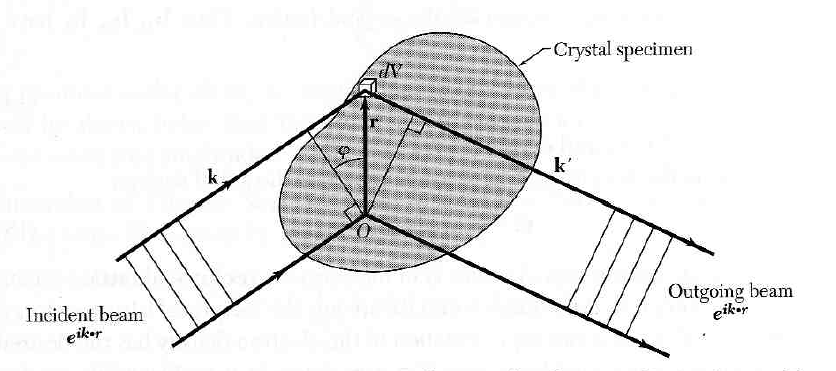
\includegraphics[width=15cm]{UvjetDiff.PNG}
       \caption{Razlika putova upadnog vala \textbf{k} u točki \textbf{O}. Razlika faznog kuta je $\mathbf{k\cdot r}= \frac{2\pi r }{\lambda}sin(\phi)$. Za difraktirani val je $-\mathbf{k'\cdot r}$. }
       \label{diffuvj}
   \end{figure}
   Sa slike \ref{diffuvj} se vidi da je razlika u faznim faktorima $e^{i\left( \mathbf{k-k'}\right)\mathbf{r}}$. Pretpostavljamo da je amplituda raspršenog vala proporcionalna s lokalnom koncentracijom elektrona $n(\mathbf{r})$. Totalna amplituda raspršenja u smjeru \textbf{k'} je 
   \begin{equation}
       F=\int dV n(\mathbf{r})e^{i\left( \mathbf{k-k'}\right)\cdot\mathbf{r}}
        =\int dV n(\mathbf{r})e^{-i \Delta\mathbf{k} \cdot \mathbf{r}}
        \label{EQ2_11}
   \end{equation}
   Gdje je $\Delta \mathbf{k}= \mathbf{k'-k}$. $\Delta \mathbf{k}$ je mjera promjene valnog vektora pri raspršenju, a obično se zove vektor raspršenja. Uvrštavanjem \ref{EQ2_6} u \ref{EQ2_11} dobivamo 
   \begin{equation}
       F= \sum_G n_G \int dV e^{i\left(\mathbf{G-\Delta k} \right)\cdot \mathbf{r}}
       \label{EQ2_12}
   \end{equation}
   F je zanemarivo malen ako se $\Delta \mathbf{k}$ značajno razlikuje od \textbf{G}. Pri elastičnom rasprošenju $\mathbf{\Delta k}=\mathbf{G}$ pa je nadalje za elastično raspršenje $\mathbf{k'=k} \rightarrow k^2={k'}^2$. Odavdje se da pokazati da je \begin{equation}
   \begin{split}
       \Delta \mathbf{k}&= \mathbf{k'-k}=\mathbf{G} \rightarrow \\
       \mathbf{k'}&=\mathbf{G+k} \rightarrow \\
       (\mathbf{k+G})^2&=k^2+2\mathbf{k\cdot G}+G^2=k^2
   \end{split}
   \label{EQ2_13}
   \end{equation}
   Odakle slijedi uvjet difrakcije:
   \begin{equation}
       2\mathbf{k\cdot G}+G^2=0.
       \label{EQ2_14}
   \end{equation}
   Isti se uvjet može zapisati kao $2\mathbf{k\cdot G}=G^2$, koristeći da je -\textbf{G} također vektor recipročne rešetke. Razmak među dviju kristalnih ravnina, $d(hkl)$ koje su okomite na \textbf{G} je jednak 
   \begin{equation}
       d(hkl)=\frac{2\pi}{\left| \mathbf{G}\right|}.
       \label{EQ2_15}
   \end{equation}
   Iz \ref{EQ2_14} uvrštavanjem $\left|\mathbf{G}\right|=\frac{2\pi}{d(hkl)}$ i $\mathbf{k}=\frac{2\pi}{\lambda} \hat{k}$ imamo 
   \begin{equation}
   2\frac{2\pi}{\lambda} sin(\theta)=\frac{2\pi}{d(hkl)} \rightarrow 2d(hkl)sin(\theta)=\lambda
       \label{EQ2_16}
   \end{equation}
   Indeksi hkl nisu identični indeksima ravnine jer hkl mogu sadržavati zajednički faktor n pa dobijemo Braggov zakon: 
   \begin{equation}
       2dsin(\theta)=n\lambda
       \label{EQ2_17}
   \end{equation}
   gdje je \textit{d} razmak među ravninama s indeksima $\frac{h}{n}$, $\frac{k}{n}$ i $\frac{l}{n}$. 
   \subsection{Laueove jednadžbe}
   Rezultat $\Delta \mathbf{k}=\mathbf{G}$ možemo izraziti drugačije. Ako taj izraz pomnožimo s vektorima $\mathbf{a_1}$, $\mathbf{a_2}$ i $\mathbf{a_3}$ dobijemo 
   \begin{equation}
   \begin{split}
       \mathbf{a_1}\cdot \Delta \mathbf{k} &= 2\pi v_1\\
       \mathbf{a_2}\cdot \Delta \mathbf{k} &= 2\pi v_2\\
       \mathbf{a_3}\cdot \Delta \mathbf{k} &= 2\pi v_3
    \end{split}
       \label{EQ2_18}
   \end{equation}
   Gornje jednadžbe \ref{EQ2_18} govore da $\Delta \mathbf{k}$ leži na stošcu oko smjera vektora $a_i$ i da bi difrakcijski uvjet bio zadovoljen $\Delta \mathbf{k}$ mora zadovoljavati sve tri jednadžbe tj. mora ležati na presjecištu svih triju stošca. 
   
\subsection{Brillouinova zona}
Čita se kao Briluen. Ako je nekome to bitno. \\
\paragraph{Definicija} Brillouinova zona je Wigner-Seitzova primitivna čelija u recipročnoj rešetci.\\
Zbog Brillouinove zone difrakcijski uvjet dobiva novu geometrijsku interpretaciju. Ako $2\mathbf{k\cdot G}=G^2$ podjelimo s 4 dobivamo:
\begin{equation}
    \mathbf{k}\cdot \frac{\mathbf{G}}{2}={\frac{G}{2}}^2
    \label{EQ2_19}
\end{equation}
Budući da radimo u recipročnom prostoru tj. prostoru \textbf{k} i \textbf{G} izaberemo vektor \textbf{G} iz ishodišta do točke recipročne rešetke te konstruiramo ravninu normalnu na središte vektora \textbf{G}. Ta ravnina formira graničnu zonu. Da bi se rendgenska zraka difraktirala, valni vektor te zrake mora imati iznos i smjer određen s \ref{EQ2_19}. Tada će difraktirana zraka biti u smjeru \textbf{k-G}. Stoga, Brillouinova zona posjeduje sve valne vektore koji će se raspršiti u kristalu. Prva Broillouinova zona je najmanji volumen koji je u potpunosti zatvorena ravninama koje su okomite i raspolavljaju vektore recipročne rešekte koji se crtaju iz ishodišta recipročne rešetke.

\subsection{Fourierova analiza baze}

   Kad je zadovoljen difrakcijski uvjet $\Delta \mathbf{k}\cdot \mathbf{G}$, amplituda raspršenja za kristal od N čelija mo
   emo napisati kao 
   \begin{equation}
       F_G=N\int_{cell}dV n(\mathbf{r})e^{-\mathbf{G\cdot r}}=N\cdot S_G,
       \label{EQ2_20}
   \end{equation}
   gdje je $S_G=\int_{cell}dV n(\mathbf{r})e^{-\mathbf{G\cdot r}}$ strukturni faktor.
   Također, $n(\mathbf{r})$ možemo pisati kao superpoziciju elektronskih koncentracija $n_j$ za svaki atom rešetke:
   \begin{equation}
       n(\mathbf{r})=\sum_{j=1}^s n_j(\mathbf{r-r_j}),
       \label{EQ2_21}
   \end{equation}
   gdje je $n_j(\mathbf{r-r_j})$ doprinos j-tog atoma koncentraciji elektrona u točki \textbf{r}. Strukturni faktor sad možemo zapisati kao 
   \begin{equation}
   \begin{split}
       S_{\mathbf{G}}&=\sum_j \int dV n_j(\mathbf{r}- \mathbf{r}_j) e^{-i\mathbf{G}\cdot \mathbf{r}}\\
       &= \sum_j e^{-i\mathbf{G}\cdot \mathbf{r}_j}\int dV n_j(\mathbf{\rho}) e^{-i\mathbf{G}\cdot \mathbf{\rho}},
   \end{split}
       \label{EQ2_22}
   \end{equation}
gdje je $\mathbf{\rho}=\mathbf{r}-\mathbf{r}_j$. \textbf{Atomski form faktor} ćemo definirati kao 
\begin{equation}
   f_j = \int dV n_j(\mathbf{\rho})e^{-i\mathbf{G}\cdot \mathbf{\rho}}.
    \label{EW2_23}
\end{equation}
Ako je $n(\mathbf{\rho})$ svojstvo atoma, onda je i $f_j$. Jednadžba \ref{EQ2_22} sad postaje
\begin{equation}
    S_{\mathbf{G}}=\sum_j f_j e^{-i\mathbf{G}\cdot \mathbf{r}}.
    \label{EQ2_24}
\end{equation}
   Za j-ti atom pišemo $\mathbf{r}_j$ kao 
   \begin{equation*}
       \mathbf{r}_j = x_j \mathbf{a}_1 + y_j \mathbf{a}_2 + z_j \mathbf{a}_3,
   \end{equation*}
   te produkt $\mathbf{G \cdot r}_j$ daje $2\pi(v_1 x_j + v_2 y_j + v_3 z_j)$, pa dobivamo strukturni faktor kao
   \begin{equation}
       S_{\mathbf{G}}=\sum_j e^{-i 2 \pi (v_1 x_j + v_2 y_j + v_3 z_j)}.
       \label{EQ2_25}
   \end{equation}
   Strukturni faktor ne mora biti realan jer je intenzitet raspršenja $S^*S$ realan, gdje je $S^*  $ kompleksno konjugirani strukturni faktor. Strukturni faktor nam daje informaciju o tome u kojoj će se ravnini u rešetci upadno zračenje uopće moći raspršiti, dok nam atomski form faktor govori o samome intenzitetu. 
   
   \begin{figure}[h!]
       \centering
       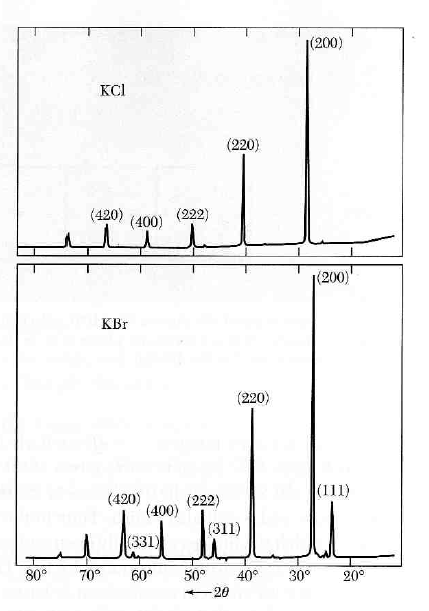
\includegraphics[width=10cm]{Difrakcija_S_g_i_AFF.png}
       \caption{Usporedba rendgenske difrakcije KCl i KBr praškastog uzorka.}
       \label{fig:DifrakSGAFF}
   \end{figure}
   
\newpage
\section{Vezanje kristala}
\textbf{Kohezivna energija} - Energija potrebna da se kristal rastavi na komponente slobodnih atoma. Često se kohezivna energija naziva i energija vezanja. Radne definicije su i kao energija potrebna da se materijal rastavi na pojedine molekule. Ne mora striktno biti 1 atom.
\subsection{Kristali inertnih plinova}
Inertni plinovi formiraju najjednostavnije kristale. Raspodjela elektrona je jako slična kao za slobodni atom. Transparentni su, slabo se vežu te imaju niska tališta. Visokih su energija ionizacije pošto im je vanjska ljuska u potpunosti popunjena. Najčešće se pakiraju u fcc rešetci. 
\begin{figure}[h!]
    \centering
    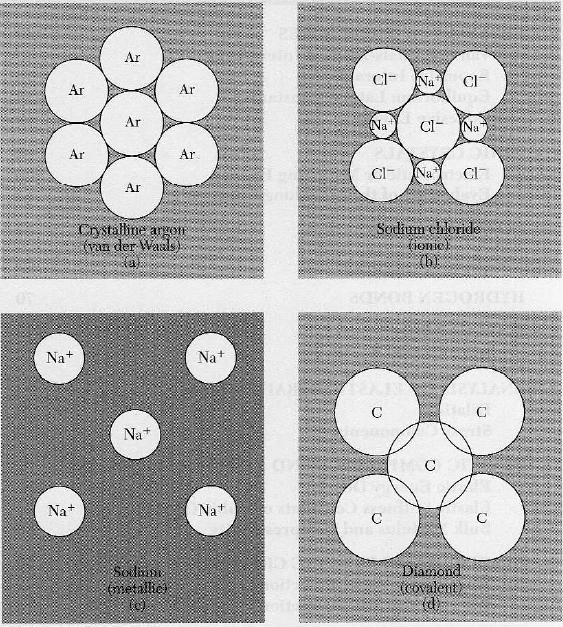
\includegraphics[width=10cm]{KristVeze1.png}
    \caption{Različiti tipovi kristalnog vezanja.}
    \label{fig:KristVeze1}
\end{figure}
\newpage
\subsubsection{Van der Waals-London interakcija - Dipol-dipol interakcija}
Van der Waals-ova ili dipol-dipol veza se stvara kad imamo 2 atoma na nekakvoj udaljenosti \textbf{R} jedan od drugog. Atomi induciraju dipolne momente jedan u drugome, te na taj način stvaraju privlačnu interakciju. 

\textbf{Model}\\ Nepertubirani Hamiltonijan gledamo kao 2 harmonijska oscilatora. Čestice osciliraju u x smjeru, $p_1$ i $p_2$ su momenti, te je konstanta sile C.
\begin{figure}[h!]
    \centering
    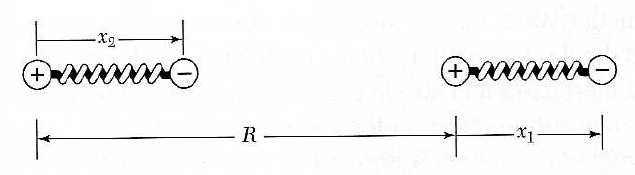
\includegraphics[width=10cm]{KristVeze2.png}
    \caption{2 atoma na udaljenosti \textbf{R}}
    \label{fig:KristVeze2}
\end{figure}

\begin{equation}
    H_0=\frac{p^2_1+p^2_2}{2m}+ \frac{C}{2}(x^2_1+x^2_2)
    \label{EQ3_1}
\end{equation}

Svaki nevezani oscilator ima frekvenciju najintenzivnije optičke apsorbcijske linije $\omega_0$, td. $C=m \omega^2_0$.

Coulombska interakcija oscilatora iz geometrije sa slike \ref{fig:KristVeze2} dobivamo kao: 
\begin{equation}
\begin{split}
    H_1&=e^2 \cdot (\frac{1}{R}+\frac{1}{R+x_1-x_2}-\frac{1}{R+x_1}-\frac{1}{R-x_2})
    &=-\frac{2e^2x_1 x_2}{R^3}
\end{split}
    \label{EQ3_2}
\end{equation}
Ukupni Hamiltonijan $H=H_0+H_1$ se može dijagonalizirati s transformacijama normalih modova: 
\begin{equation}
    x_1=\frac{x_s+x_a}{\sqrt{2}}\text{ i } x_2=\frac{x_s-x_a}{\sqrt{2}}
\end{equation}
Slično vrijedi i za momente $p_1$ i $p_2$:
\begin{equation}
    p_1=\frac{p_s+p_a}{\sqrt{2}}\text{ i } p_2=\frac{p_s-p_a}{\sqrt{2}}
\end{equation}
Uvrstimo zadnje dvije jednadžbe u ukupni Hamiltonijan i dobivamo: 
\begin{equation}
    H=\left(\frac{p^2_s}{2m}+x^2_s\left[\frac{C}{2}-\frac{e^2}{R^3} \right]  \right)+ \left( \frac{p^2_a}{2m}+x^2_a\left[\frac{C}{2}+ \frac{e^2}{R^3}\right] \right)
\end{equation}
Frekvencije vezanog oscilatora su onda: 
\begin{equation}
\begin{split}
      \omega &= \sqrt{\frac{C \pm \frac{2e^2}{R^3}}{m}}\\
      &=\omega_0\left[1\pm\frac{1}{2}\frac{2e^2}{CR^3}-\frac{1}{8}\left(\frac{2e^2}{CR^3}\right)^2+... \right]\\
      &= \sqrt{\frac{C}{m}}\sqrt{1\pm \frac{2e^2}{CR^3}}
\end{split}
  \label{EQ3_3}
\end{equation}
Gdje je $\omega_0 = \sqrt{\frac{C}{m}}$. Energija osnovnog stanja je $U'=\frac{\hbar}{2}(\omega_s+\omega_a)$, dok je energija nevezanih oscilatora $U_0=2\frac{1}{2}\hbar \omega_0$. Time je energija umanjena za 
\begin{equation}
\Delta U = \frac{\hbar}{2}(\Delta \omega_s + \Delta \omega_a)= -\frac{A}{R^6},
\label{EQ3_4}
\end{equation}
gdje je $A=\frac{\hbar \omega_0 e^2}{2C^2}$.
\newpage
\subsubsection{Repulzivna interakcija (odbojna interakcija)}
Približavanjem atoma dolazi do repulzivne interakcije među njima. Uglavnom zbog Paulijevog principa. Dva fermiona se ne mogu naći u istom kvantom stanju, tj, barem jedan od 4 kvantna broja se moraju razlikovati. Atomi s popunjenim ljuskama će osječati takozvani efekt preklapanja ljuski što dovodi do egzcitacije elektrona u više stanje od jednog od atoma. Time se povečava energija sustava i nastaje repulzivna sila među njima. Eksperimentalno se pokazalo da $\frac{B}{R^12}$ oblik takve interakcije. Zajedno s jednadžbom \ref{EQ3_4} dobivamo Lennard-Jonesov potencijal
\begin{equation}
    U(R)=4\epsilon\left[\left( \frac{\sigma}{R}\right)^12-\left(\frac{\sigma}{R}\right)^6\right].
    \label{EQ3_5}
\end{equation}
Tu smo zamjenili $A=4\epsilon \sigma^6$ i $B=4\epsilon \sigma^12$.
\subsubsection{Ravnotežne konstante rešetke}
Ako ignoriramo kinetičke energije, kohezivna energija inertnog plina je samo suma L.J. potencijala (\ref{EQ3_5}) po kristalnim parovima: 
\begin{equation}
    U_{tot}=\frac{N}{2}4\epsilon\left[\sum_j \left( \frac{\sigma}{p_{ij}R}\right)^12-\sum_j\left(\frac{\sigma}{p_{ij}R}\right)^6\right],
    \label{EQ3_6}
\end{equation}
gdje su $p_{ij}R$ udaljenosti između i-tog i j-tog atoma, zapisano momoću udaljenosti najbližih susjde R. Faktor $\frac{1}{2}$ dolazi zbog dvostrukog prebrojavanja. Dobivamo faktore najbližih susjeda za fcc rešetku 
\begin{equation}
    \sum_j p^{-12}_{ij} = 12,13188 \text{, i } \sum_j p^{-6}_{ij}=14,45392.
    \label{Konstante1}
\end{equation}
Deriviranjem jednadžbe \ref{EQ3_6} po R i uvrštavanjem \ref{Konstante1} za fcc strukturu dobivamo 
\begin{equation}
    \frac{dU_{tot}}{dR}=0=-2N\epsilon\left[ 12\cdot12,13188 \frac{\sigma^12}{R^13}-6\cdot14,45392 \frac{\sigma^6}{R^7} \right].
    \label{EQ3_7}
\end{equation}
Dobivamo traženi rezultat koji ćemo koristiti sad za dobivanje kohezivne energije, $\frac{R_0}{\sigma}=1,09$. Kohezivnu energiju dobivamo jednostavnim uvrštavanjem prijašnjeg rezultata $\frac{R_0}{\sigma}=1,09$ i \ref{Konstante1} u L.J. potencijal: 
\begin{equation}
    U_{tot}= -2,15\cdot 4 \cdot \epsilon.
\label{EQ3_8}
\end{equation}
\subsection{Ionski kristali}
Napravljeni su od pozitivnih i negativnih iona. Ionska veza nastaje zbog elektrostatske interakcije suprotno nabijenih čestica. Raspodjela elektrona je više mane sferno simetrična, sve do područja kontakta s drugim ionom, gdje dolazi do distorzije. Promatrat ćemo elektrostatsku interakciju da bi otkrili što se događa s energijom vezanja ionskih kristala.
\vfill
\textbf{Elektrostatska/Madelung energija} - Elektrostatska interakcija je dalekodosežna i poznatog nam je oblika $\pm \frac{q^2}{r}$. Za istoznačne naboje je odbojna, za suprotne je privlačna. Glavni doprinos vezanja ionskih kristala je tzv. \underline{Madelung energija}.
\begin{equation}
    U_i=\sum_j U_{ij},
\end{equation}
gdje je $U_{ij}$ interakcija i-tog i j-tog iona, a suma ide po svim ionima osim i=j. Pretpostavljamo da $U_{ij}$ možemo pisati kao $\lambda e^{-\frac{r}{\rho}}$, gdje su $\lambda$ i $\rho$ empirijski parametri, te s Coulmbovim potencijalom. Dobivamo sad 
\begin{equation}
    U_{ij}=\lambda e^{-\frac{r}{\rho}} \pm \frac{q^2}{r}.
    \label{EQ3_9}
\end{equation}
Repulzivni član dolazi zbog činenice da svaki ion odupire preklapanju raspodjela elektrona sa susjednim ionima. Ignorirati ćemo površinske efekte i napisati ćemo $U_{tot}$ za kristale od N molekula kao $U_{tot}=NU_i$. Opet ćemo uvesti $p_{ij}$ t.d. $r_{ij}=p_{ij}R$:

\begin{equation}
U_{i j}=\left\{\begin{array}{l}
\lambda \exp (-R / p)-\frac{q^{2}}{R}; \text{najbliži susjedi} \\
\pm \frac{1}{p_{i j}} \frac{q^{2}}{R}; \text{inače}
\end{array}\right.
\label{EQ3_10}
\end{equation}
Odnosno,
\begin{equation}
    U_{tot}=NU_i=N\left(z\lambda e^{\frac{-R}{\rho}}-\alpha \frac{q^2}{R}\right),
    \label{EQ3_11}
\end{equation}
gdje je $\alpha=\sum_j \frac{(\mp)}{p_{ij}}$, i z je broj najbližih susjeda. Vrijednost $\alpha$ je jako bitna u teoriji ionskih kristala. Tražimo sad minimum prijašnjeg potencijala \ref{EQ3_11}
\begin{equation}
\begin{split}
    \frac{dU_{tot}}{dR}&=0\\
    N\frac{dU_i}{dR}&=-\frac{Nz\lambda}{\rho}e^{-\frac{r}{\rho}}+\frac{N\alpha q^2}{R^2}=0\\
    R^2_0 e^{\frac{R_0}{\rho}}&=\frac{\rho \alpha q^2}{z\lambda}
\end{split}
\label{EQ3_12}
\end{equation}
Odavdje dobivamo $R_0$ ako znamo $\lambda$ i $\rho$. Za 2N iona dobivamo ukupnu energiju rešetke kao:
\begin{equation}
    U_{tot}=-\frac{N\alpha q^2}{R_o}\left(1-\frac{\rho}{R_0}\right),
    \label{EQ3_13}
\end{equation}
gdje možemo $-\frac{N\alpha q^2}{R_o}$ definirati kao Madelung energiju.

\subsection{Kovalentni kristali}

\newpage
\subsubsection{Kratki sažetak}
\begin{figure}[h!]
    \centering
    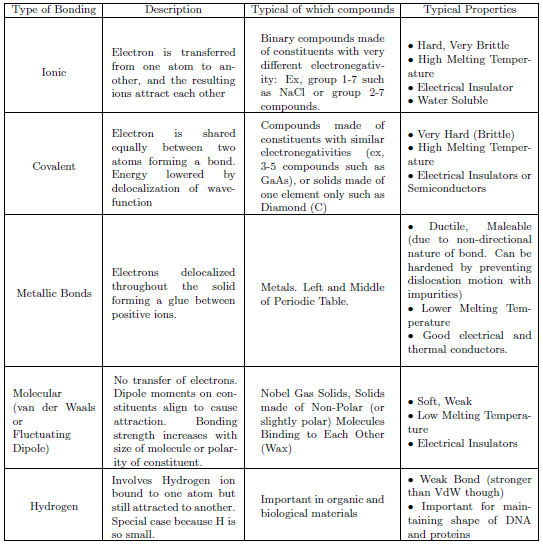
\includegraphics[width=\linewidth]{Tablica.png}
    \caption{Slika tablice iz 'Lecture Notes for Solid State Physics' koju je napisao Professor Steven H. Simon. Ukratko su napisane sve bitne stvari koje smo do sad naveli.}
    \label{fig:TablicaSažetak}
\end{figure}
\newpage
\section{Fononi I. Vibracije kristala}

\section{Fononi II. Termička svojstva}

\section{Fermijev plin slobodnih $e^-$}

\section{Energijske vrpce}

\newpage
\section*{Disclamer}
Neke slike su preuzete s interneta, neke su preuzete iz knjige Introduction to Solid State Physics od Charles Kittela. Nisam stavio reference na njih jer mi se nije dalo.
\end{document}
